\chapter{Introduction to Arduino}

\section{Open Hardware}
\emph{"There's a fine line between open source and stupidity"}, says Massimo Banzi to a reporter from Wired Magazine while having dinner at a restaurant in Milan. 

Banzi is the man behind Arduino, an open hardware platform. The open about it relates to the fact that the device's manufacturing schematics, programming language and software development environment are free and open source. This basically means that everyone interested on building hardware-coupled solutions may take an Arduino board's schematics, modify it at will, send the new design to a China manufacturer and get the final product back home for around \EUR{10}~\cite{wiredOpenHardware}.

Open hardware is supported by a variety of available licenses (like open software with LGPL, GPL, Copyleft, and others) that ensure that the protected platform can be copied, enhanced and even sold, but always recognizing the original authors. It also ensures that the resulting products are open as the original.

\section{The Arduino Platform}
Arduino was developed to teach Interaction Design~\cite{banzi2008getting}, that meant that it required the ability to sense the surroundings and do something about it.

The platform is equipped with simple digital and analog input/output interfaces, that can be programmed to sense or react to some events. Figure~\ref{fig:ArduinoBoard} shows the Arduino Duemilanove board.

\begin{figure}[htbp]
  \centering
  \includegraphics[width=0.7\linewidth]{figures/duemilanove.eps}
  \caption{Arduino Duemilanove board
  \label{fig:ArduinoBoard}}
\end{figure}

There are numerous sensors and actuators that work with Arduino. In relation to sensors: temperature, air pollution, light, GPS modules and sound are among the popular; as LEDs, speakers and digital/analog outputs are common actuators. Also, interfaces like buttons can be programmed and used as a human interactive input.

The design and electrical components of the Arduino board are available for anyone~\cite{Arduino}. Figure~\ref{fig:Arduino_schematics} shows the connections layout of the Duemilanove model (compare with Figure~\ref{fig:ArduinoBoard}).

\begin{figure}[htbp]
  \centering
  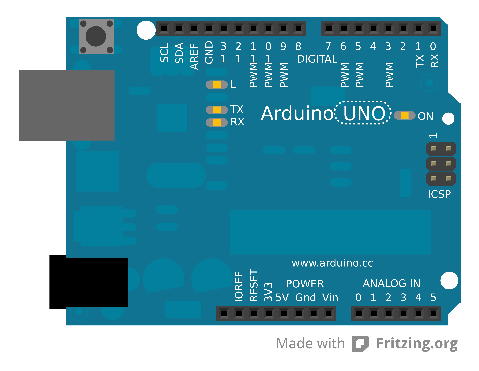
\includegraphics[width=0.7\linewidth]{figures/duemilanove_layout_NEW.eps}
  \caption{Arduino Duemilanove board: layout
  \label{fig:Arduino_schematics}}
\end{figure}